\documentclass{beamer}
\usepackage{hyperref}
\hypersetup{
	colorlinks,
	citecolor=white,
	filecolor=white,
	linkcolor=white,
	urlcolor= cyan
}

\usetheme[progressbar=foot, background=dark]{metropolis}  
\setbeamertemplate{frame footer}{Ankit Pant - 2018201035}

\title{\centering Image Super-resolution using \\ Generative Adversarial Networks\\ \vspace{2mm} \normalsize{PG - Independent Study } \\ \vspace{-5mm}}
\author{Ankit Pant \\ 2018201035 \\ 
	\textit{M.Tech. Computer Science \& Engineering} \\
	International Institute of Information Technology, Hyderabad \\
	Supervised by: Dr. Pawan Kumar
	}
\date{}
\begin{document}
\begin{frame}[plain]
    \maketitle
\end{frame}
\begin{frame}{Outline}
	\setbeamertemplate{section in toc}[sections numbered]
	\tableofcontents
\end{frame}

\section{Introduction}
	\begin{frame}{Introduction}
		\begin{itemize}
			\item Artificial Intelligence (AI) and Machine Learning being used for a large number of applications
			\item Generative Adversarial Networks among various models used in AI and Machine Learning (ML)
			\item  Image Super-resolution is one such application
			\item PG-Independent Study aims to cover GANs and Image Super-resolution (in moderate detail) 
			\item Study includes creating ML model and Web App  to use the model
		\end{itemize}
	\end{frame}

\section{Literature Review}
	\begin{frame}{Generative Adversarial Networks (GANs)}
		\begin{itemize}
			\item Generative Adversarial Networks (GANs) -- combination of two  models: generator and discriminator model working in tandem
			\item Generator model:
			\begin{itemize}
				\item It is responsible for generating images (usually from noise)
			\end{itemize}
			\item Discriminator model:
			\begin{itemize}
				\item It is responsible to determine whether the image was originally available or generated by the generator 
			\end{itemize}
			\item Various Types of GANs include:
			\begin{itemize}
				\item Deep Convolutional GANs (DCGAN)
				\item Wasserstein GAN (WGAN)
				\item Softmax GAN
			\end{itemize}
		\end{itemize}
		
	\end{frame}

	\begin{frame}{Sample Training Phrase of a GAN}
		\begin{itemize}
			\item The generator tries to recreate original image from noise
			\item This image is then input to discriminator which tries to identify whether it was generated
			\item The generator then again improves on the generated images
			\item The discriminator again determines whether the images was generated or not
			\item This process is repeated until the discriminator can no longer determine whether the image was generated or not $P(generated) = P(original) = 0.50$
			\item Both the generator and discriminator may be pre-trained to improve performance
		\end{itemize}
	\end{frame}

	
	\begin{frame}{Image Super-resolution}
		
		\begin{itemize}
			\item 	\textbf{Image Super-resolution:} Conversion of (one or more) low resolution images into a high resolution image 
			\item Benefits of increasing image resolution:
			\begin{itemize}
				\item The resultant image is larger
				\item It provides more details
				\item Can be used to improve image quality as well as video quality
			\end{itemize}
			\item Application of image super-resolution
			\begin{itemize}
				\item Enhancing photographs and self-portraits of people
				\item Enhancing surveillance footage
				\item Enhancing medical diagnostic images
				\item Enhancing astronomical and remotes sensing images
				\item Enhancing low resolution videos
			\end{itemize}
		\end{itemize}
	\end{frame}
	
	\begin{frame}{Image Super-resolution - Technique}
		\begin{itemize}
			\item \textbf{Single-frame Super-resolution}
			\begin{itemize}
				\item Traditional resolution enhancement  - includes smoothing, interpolation and sharpening
				\item Estimates detail that is not present
				\item Training-set used to learn details of images at low resolution
				\item These learned relationships used to predict details of other images
			\end{itemize}
			\item \textbf{Multi-frame Super-resolution}
			\begin{itemize}
				\item Works if multiple low resolution images are available of the same scene
				\item Each image is naturally shifted with sub-pixel precision
				\item Works when each of the images have different sub-pixel shifts
			\end{itemize}
		\end{itemize}
	\end{frame}


\section{Methodology}
	\begin{frame}{Implementing Single-frame Super-resolution}
		\begin{itemize}
			\item Approach consists of two steps:
			\begin{enumerate}
				\item Creating and training ML model
				\item Creating the Web application to use the model
			\end{enumerate}
			\item The code is in the form of Jupyter Notebook
			\item Google Colab -- the platform to train and test
			the model
			\item ML model currently can scale low-resolution images to a resolution of 512 x 512 pixels
			\item Measures to Compare Images:
			\begin{itemize}
				\item Multi Scale Structural Similarity (MS-SSIM)
				\item Mean Squared Error (MSE)
				\item Peak Signal to Noise Ratio (PSNR)
				\item L1 distance
			\end{itemize}
		\end{itemize}
	\end{frame}

	\begin{frame}{Overview of the algorithm}
		\begin{enumerate}
			\item Convert high resolution images to low resolution images
			\item Train generator model on this dataset. Store resultant generated images
			\item Train discriminator model on generated and original images
			\item Combine generator and discriminator in GAN and train it 
			\item Save the model as well as generated images
			\item Use model to upsample images to size 512 x 512
			\item Run the model on test dataset
			\item Import the saved models to the web application
		\end{enumerate}
	\end{frame}

	\begin{frame}{Architecture of ML model}
		\begin{itemize}
			\item Generator:
			\begin{itemize}
				\item UNet model
				\item ResNet34 as base architecture
				\item Mean Squared Error (MSE) as loss function
			\end{itemize}
			\item Discriminator:
			\begin{itemize}
				\item basic gan\_critic model (from fastai)
				\item Cross Entropy as loss function
			\end{itemize}
			\item Up-sampler:
			\begin{itemize}
				\item UNet model
				\item VGG16 as base architecture
				\item Mean Squared Error (MSE) as loss function
			\end{itemize}
		\end{itemize}
	\end{frame}

	\begin{frame}{Architecture of ML model}
		\vspace{3mm}
		\begin{figure}[htbp]
			\centerline{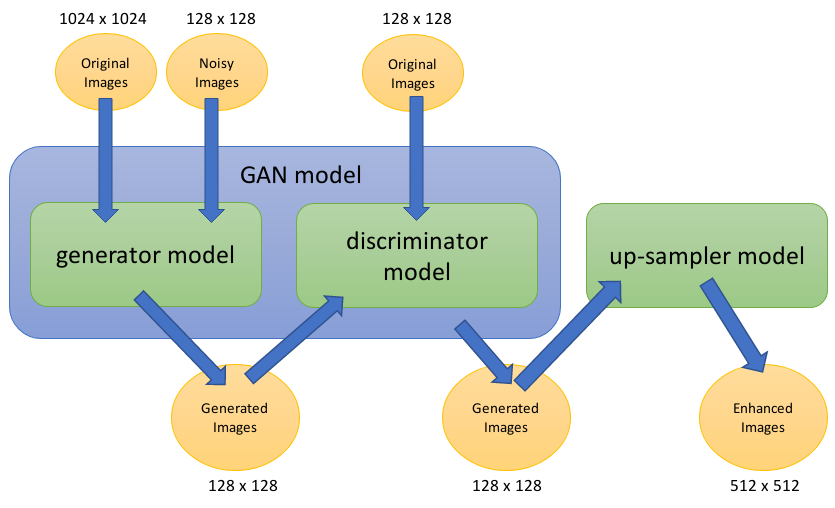
\includegraphics[width=25em]{arch_srgan.png}}
			\caption{Architecture of ML model}
			\label{arch-fig}
		\end{figure}
	\end{frame}

	\begin{frame}{Training and Test Datasets}
		\begin{itemize}
			\item Training dataset (high quality):
			\begin{itemize}
				\item 1600 images
				\item Flickr-Faces-HQ Dataset
				\item Created originally as a benchmark for GANs 
			\end{itemize}
			\vspace{3mm}
			\item Test dataset (low quality):
			\begin{itemize}
				\item 300 images
				\item  Selfie Data Set
			\end{itemize}
		\end{itemize}
	\end{frame}

	\begin{frame}{Creating Web Application}
		\begin{itemize}
			\item The Web Application has been created in Python
			\item Deployed using Docker
			\item Allows user to pick low resolution images
			\item enhances them to 512 x 512 resolution
		\end{itemize}
		\vspace{3mm}
		\begin{figure}[htbp]
			\centerline{
\includegraphics[width=18em]{webapp_ui1.png}}
			\caption{Web application UI (no image chosen)}
			\label{appui1-fig}
		\end{figure}
	\end{frame}

	\begin{frame}{Creating Web Application}
		\begin{figure}[htbp]
			\centerline{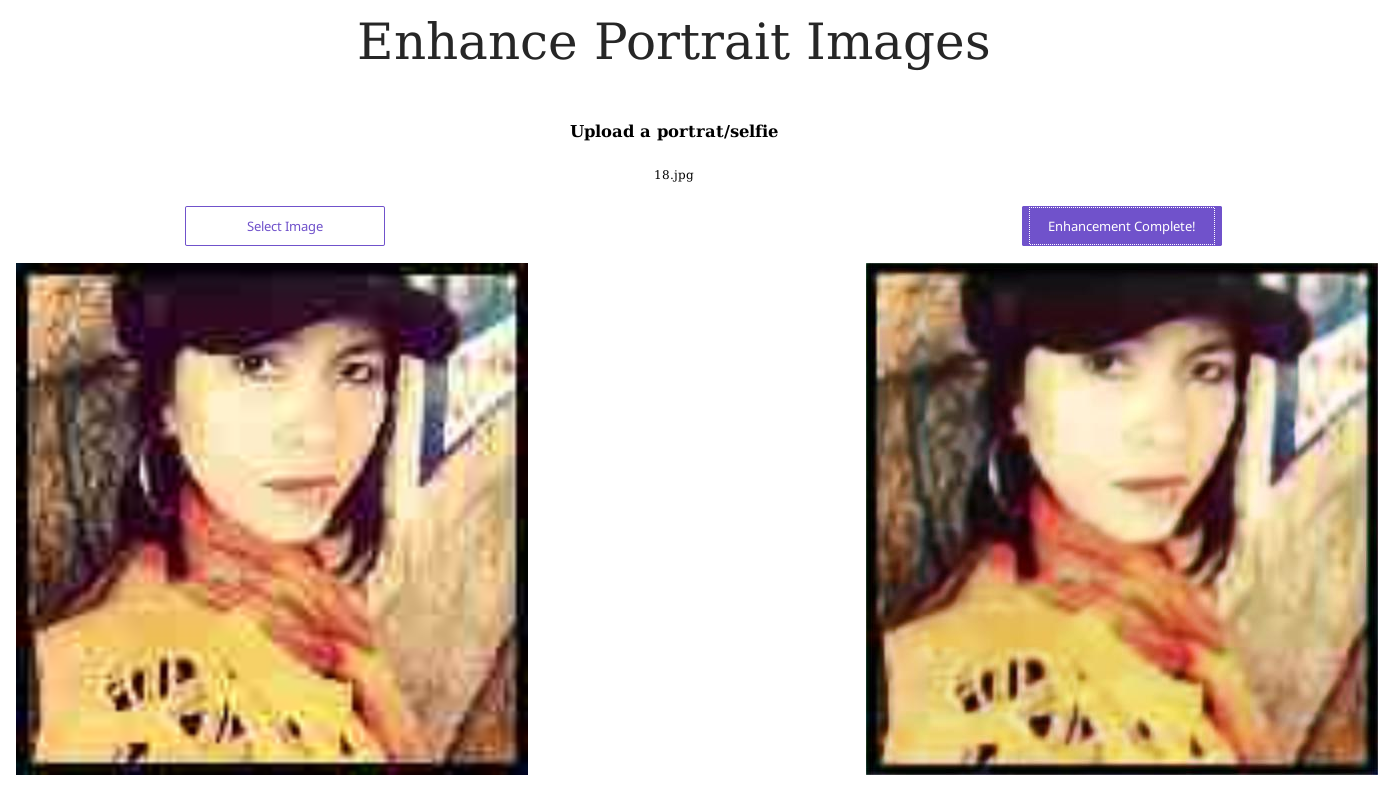
\includegraphics[width=25em]{webapp_ui2.png}}
			\caption{Web application UI (after enhancing image)}
			\label{appui2-fig}
		\end{figure}
	\end{frame}
	

\section{Experimentation}
	\begin{frame}{Experimental Setup}
		\begin{itemize}
			\item Training Environment - Google Colab:
			\begin{itemize}
				\item RAM: 25.51 GB
				\item VRAM: 12 GB
				\item Disk Space: 358.27 GB
			\end{itemize}
			\item Approximate time required to train various components:
			\begin{itemize}
				\item Generator model: 13 minutes
				\item Discriminator model: 18 minutes
				\item GAN: 48 minutes
				\item Up-sampler: 135 minutes
			\end{itemize}
		\end{itemize}
	\end{frame}

\section{Results}
	\begin{frame}{Comparison: Low-res images vs generated images}
		\begin{itemize}
			\item Both low res images and generated images compared to original images
		\end{itemize}
		\begin{table}[htbp]
			\caption{Comparison between low-res and initially generated images}
			\begin{center}
				\begin{tabular}{| p{0.2cm}| p{2cm}| p{1.5cm}|p{1.8cm}|p{1.5cm}|p{1.8cm}|}
					
					\hline
					
					& Image type      & average SSIM & average MSE  & average PSNR & average L1 \\ \hline
					
					1      & Low-res Image     & 0.127138     & 25652.10 & 4.2958    & 3.603e+06     \\ \hline
					
					2      & Generated Image & 0.135904     & 25757.22 & 4.3048    & 3.611e+06     \\ \hline
					
					
				\end{tabular}
				\label{tab1}
			\end{center}
		\end{table}
	\end{frame}
	
	\begin{frame}{Comparison: Low-res images vs enhanced images}
		\begin{itemize}
			\item Both low res images and generated images compared to original images
		\end{itemize}
		\begin{table}[htbp]
			\caption{Comparison between low-res and enhanced images}
			\begin{center}
				\begin{tabular}{| p{0.2cm}| p{2cm}| p{1.5cm}|p{1.8cm}|p{1.5cm}|p{1.8cm}|}
					
					\hline
					
					& Image type     & average SSIM & average MSE  & average PSNR & average L1 \\ \hline
					
					1      & Noisy Image    & 0.308175     & 25258.53 & 4.3702     & 5.720e+07     \\ \hline
					
					2      & Enhanced Image & 0.340402     & 24976.29 & 4.4560     & 5.675e+07     \\ \hline
					
				\end{tabular}
				\label{tab2}
			\end{center}
		\end{table}
	\end{frame}

	\begin{frame}{Sample Results using VGG up-sampler}
		\begin{figure}[htbp]
			\centerline{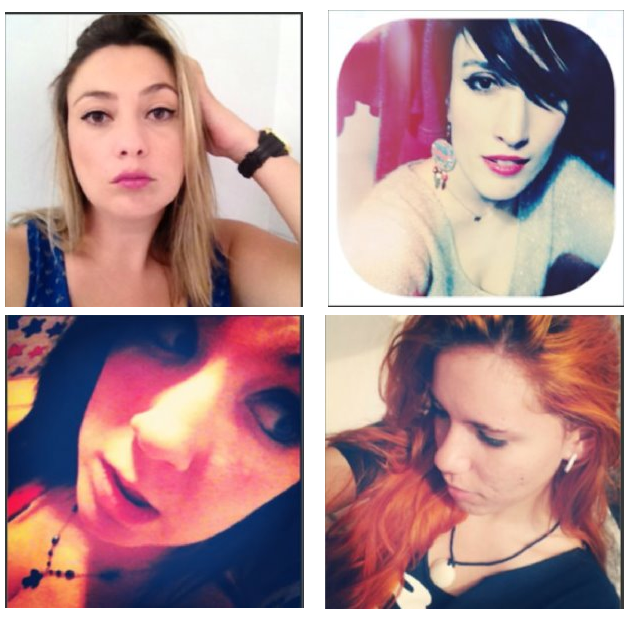
\includegraphics[width=17em]{res_vgg.png}}
			\caption{Results of image enhancement (vgg)}
			\label{res-fig}
		\end{figure}
	\end{frame}

	\begin{frame}{Sample Results using basic up-sampler (app)}
	\begin{figure}[htbp]
		\centerline{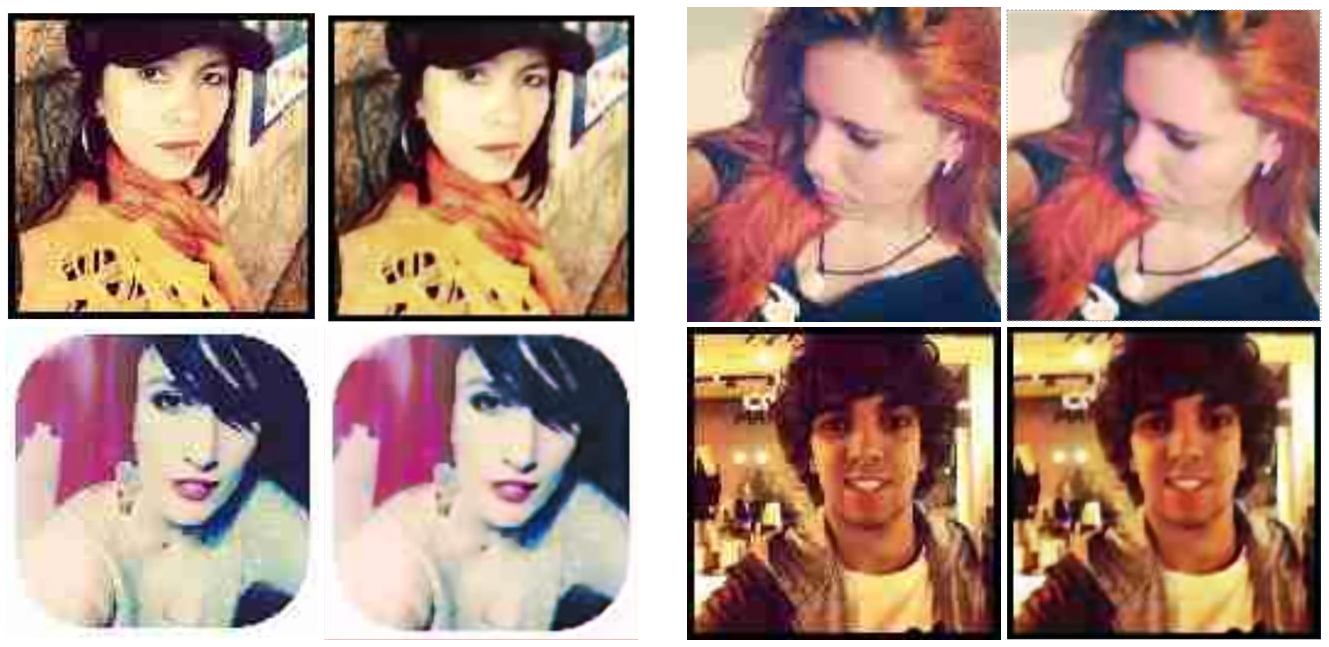
\includegraphics[height=12em, width=20em]{res_2.png}}
		\caption{Results of image enhancement (web-app)}
		\label{res2-fig}
	\end{figure}
\end{frame}


\section{Conclusion}
	\begin{frame}{Conclusion}
		\begin{itemize}
			\item AI and ML models getting better -- can even outperform humans
			\item This Independent Study applies developments in ML to enhance low resolution images
			\item ML models created that can be imported by other applications
			\item ML models created that can be used for transfer learning
			\item Created Web application that can perform image enhancements
			\item Can have commercial application as well
		\end{itemize}
	\end{frame}


\section{Drawbacks}
	\begin{frame}{Drawbacks of current implementation}
		\begin{itemize}
			\item Maximum output resolution of 512 x 512
			\item Works only for low resolution images
			\item Web application unable to use VGG based up-sampler
			\item Model trained on relatively small dataset
			\item Can have extra smoothing effect
			\item Output of images containing certain scenes overexposed
		\end{itemize}
	\end{frame}



\section{Future Scope}
	\begin{frame}{Future Scope}
		\begin{itemize}
			\item Current Implementation
			\begin{itemize}
				\item Output resolution may be increased
				\item Training loop can be extended for better predictions
				\item Size of training dataset can be increased
				\item More complex underlying architectures can be used
				\item Web application can be deployed on cloud (e.g. AWS)
			\end{itemize}
			\item Other Approaches:
			\begin{itemize}
				\item Using perceptual loss functions
				\item Using Automated Texture Analysis
				\item Incremental training
					\begin{enumerate}
						\item Train 64x64 images, followed by
						\item Train 128x128 images, followed by
						\item Train 256x256 images, etc.
					\end{enumerate}
			\end{itemize}
		\end{itemize}
	\end{frame}

\section{References}
	\begin{frame}[allowframebreaks]{References}
		
		\begin{thebibliography}{30}
		\bibitem{b1} {Goodfellow}, Ian J. and {Pouget-Abadie}, Jean and {Mirza}, Mehdi and {Xu}, Bing and {Warde-Farley}, David and {Ozair}, Sherjil and {Courville}, Aaron and {Bengio}, Yoshua, ``Generative Adversarial Nets'', arXiv e-prints, \url{https://arxiv.org/pdf/1406.2661.pdf}
		\bibitem{b2} ``Generative Adversarial Network'', Wikipedia, the free encyclopedia, \url{https://en.wikipedia.org/wiki/Generative\_adversarial\_network}
		\bibitem{b3} Alec Radford, Luke Metz, Soumith Chintala, ``Unsupervised Representation Learning with Deep Convolutional Generative Adversarial Networks'', arXiv e-prints, \url{https://arxiv.org/pdf/1511.06434.pdf}
		\bibitem{b4} Martin Arjovsky, Soumith Chintala, Léon Bottou, ``Wasserstein GAN'', arXiv e-prints, \url{https://arxiv.org/pdf/1701.07875.pdf}
		\bibitem{b5} Min Lin, ``Softmax GAN'', arXiv e-prints, \url{https://arxiv.org/pdf/1704.06191.pdf}
		\bibitem{b6}  Kevin Su, ``Introduction to Image Super-resolution'', \url{http://www.cs.utsa.edu/~qitian/seminar/Fall04/superresolution/SR_slides_xsu.pdf} 
		\bibitem{b7} Jeremy Howard et al, ``fastai'', \url{https://docs.fast.ai/}, \url{https://www.fast.ai/}
		\bibitem{b8} NVlabs, ``Flickr-Faces-HQ Dataset (FFHQ)'', \url{https://github.com/NVlabs/ffhq-dataset}
		\bibitem{b9} Center for Research in Computer Vision, ``Selfie Data Set'', University of Central Florida \url{https://www.crcv.ucf.edu/data/Selfie/}
		\bibitem{b10} Olaf Ronneberger, Philipp Fischer, Thomas Brox, ``U-Net: Convolutional Networks for Biomedical Image Segmentation'', arXiv e-prints, \url{https://arxiv.org/pdf/1505.04597.pdf}
		\bibitem{b11} Kaiming He, Xiangyu Zhang, Shaoqing Ren, Jian Sun, ``Deep Residual Learning for Image Recognition'', arXiv e-prints,  \url{https://arxiv.org/pdf/1512.03385.pdf}
		\bibitem{b12} ``Mean squared error'', Wikipedia, the free encyclopedia, \url{https://en.wikipedia.org/wiki/Mean_squared_error}
		\bibitem{b13} ``Cross entropy'', Wikipedia, the free encyclopedia, \url{https://en.wikipedia.org/wiki/Cross_entropy}
		\bibitem{b14} Neurohive, ``VGG16 – Convolutional Network for Classification and Detection'', \url{https://neurohive.io/en/popular-networks/vgg16/}
		\bibitem{b15} ``Structural similarity'', Wikipedia, the free encyclopedia, \url{https://en.wikipedia.org/wiki/Structural_similarity#Multi-Scale_SSIM}
		\bibitem{b16} ``Peak signal-to-noise ratio'', Wikipedia, the free encyclopedia, \url{https://en.wikipedia.org/wiki/Peak_signal-to-noise_ratio}
		\bibitem{b17} ``Least absolute deviations'', Wikipedia, the free encyclopedia, \url{https://en.wikipedia.org/wiki/Least_absolute_deviations}
		\bibitem{b18} ``L1 norm'', Wikipedia, the free encyclopedia, \url{https://en.wikipedia.org/w/index.php?title=L1_norm&redirect=no}
		\bibitem{b19} Christian Ledig, Lucas Theis, Ferenc Huszar, Jose Caballero, Andrew Cunningham, Alejandro Acosta, Andrew Aitken, Alykhan Tejani, Johannes Totz, Zehan Wang, Wenzhe Shi, ``Photo-Realistic Single Image Super-Resolution Using a Generative Adversarial Network'', arXiv e-prints, \url{https://arxiv.org/pdf/1609.04802.pdf}
		\bibitem{b20} Mehdi S. M. Sajjadi, Bernhard Schölkopf, Michael Hirsch, ``EnhanceNet: Single Image Super-Resolution Through Automated Texture Synthesis'', arXiv e-prints, \url{https://arxiv.org/pdf/1612.07919.pdf}
		\end{thebibliography}
	
	\end{frame}

\end{document}
